%%================================================
%% Chapter 2
%%================================================
\chapter{ทฤษฎีหรืองานที่เกี่ยวข้อง}
%\label{literature}
\label{chapter2}

\section{API}
    API หรือ Application Programming Interface คือ ช่องทางการเชื่อมต่อช่องทางหนึ่ง
ที่ทําการเชื่อมต่อกับเว็บไซต์ผู้ให้บริการ API จากที่ตั้งอื่น ทําหน้าที่เป็นตัวกลางทําให้โปรแกรมประยุกต์
เชื่อมต่อกับโปรแกรมประยุกต์อื่น หรือเชื่อมการทํางานเข้ากับระบบปฏิบัติการ (Operating System)
ทํางานตามการตอบรับของ input และ output
   



\subsection{รูปแบบของ API}
    ในส่วนของรูปแบบของ API ที่พบบ่อยและใช้ในชีวิตประจําวัน แบ่งได้เป็น 3 รูปแบบ คือ
    \begin{enumerate}
    \item Application คือ API ในรูปแบบ apps ที่ใช้ได้ผ่านสมาร์ตโฟนหรือโปรแกรมซอฟต์แวร์อื่น ๆ
    \item Programming คือ นักพัฒนา (Developer) ใช้ API ในการเขียนซอฟต์แวร์ต่าง ๆ
    \item Interface คือ รูปแบบที่ต้องใช้ในการติดต่อกับแอปพลิเคชัน
\end{enumerate}

\subsection{ลักษณะการทํางานของ API}
    ลักษณะการทํางานของ API ลักษณะการทํางานของ API สามารถเปรียบเทียบได้กับการ
สั่งเครื่องดื่มที่บาร์ ที่มีสิ่งที่ต้องทําก่อนสั่งคือการดูเมนูเครื่องดื่ม และเลือกเครื่องดื่มที่จะสั่ง ในส่วนนี้
เปรียบได้กับตัว API ดังนี้
    \begin{itemize}[\textbullet]
        \item ตัวเมนูคือ interface และรายชื่อเครื่องดื่มทั้งหมดบนเมนูเป็นสิ่งที่พนักงานผสมเครื่องดื่ม (Bartender)
            สามารถที่จะเสิร์ฟได้ ถ้าสั่งเครื่องดื่มที่มีรายชื่ออยู่บนเมนู ก็จะได้รับเครื่องดื่มนั้น แต่ถ้าสั่งเครื่อง
            ดื่มที่อยู่นอกเมนู เช่น ในเมนูมี gin martini แต่เลือกที่จะสั่ง vodka พนักงานผสมเครื่องดื่ม
            จะไม่สามารถเสิร์ฟเครื่องดื่มที่สั่งได้ เนื่องจาก ตัวพนักงานไม่สามารถที่จะหาวัตถุดิบสําหรับทํา
            vodka มาเสิร์ฟได้ เพราะไม่ได้เตรียมตัวมาก่อน แต่ในบางกรณี เช่น หากต้องการจะสั่งเครื่องดื่ม
            gin martini มาดื่มที่บ้าน โดยปกติแล้วจะทําการใช้บริการส่งถึงบ้าน (Delivery) เลือกเครื่องดื่ม
            gin martini ที่อยู่บนเมนู และเมื่อทําการสั่งเสร็จสิ้น จะมีคนบอกเครื่องดื่มที่สั่งให้กับพนักงาน
            ผสมเครื่องดื่ม และพนักงานจะทําการผสมเครื่องดื่ม martini และให้พนักงานส่งของนําเครื่อง
            ดื่มมาส่งที่บ้าน นี่คือตัวอย่างของ additional service (Delivery) ที่อยู่บน API (เมนู)
        \item โดยสรุปแล้ว API สามารถช่วยเหลือให้แอปพลิเคชันของผู้ใช้หนึ่ง ๆ สามารถรับข้อมูลที่ระบุเป็น
            ชนิดนั้น ๆ จากแอปพลิเคชันของผู้ใช้อีกฝ่ายหนึ่งได้ แต่ถ้า API ไม่สามารถรองรับชนิดข้อมูลนั้น
            ได้ ก็จะไม่สามารถที่จะช่วยดึง ข้อมูลจากสิ่งที่ไม่รู้จัก (สิ่งที่อยู่นอกเมนู) ได้
    \end{itemize}
    \begin{figure}[H]
            \centering
                \centering
                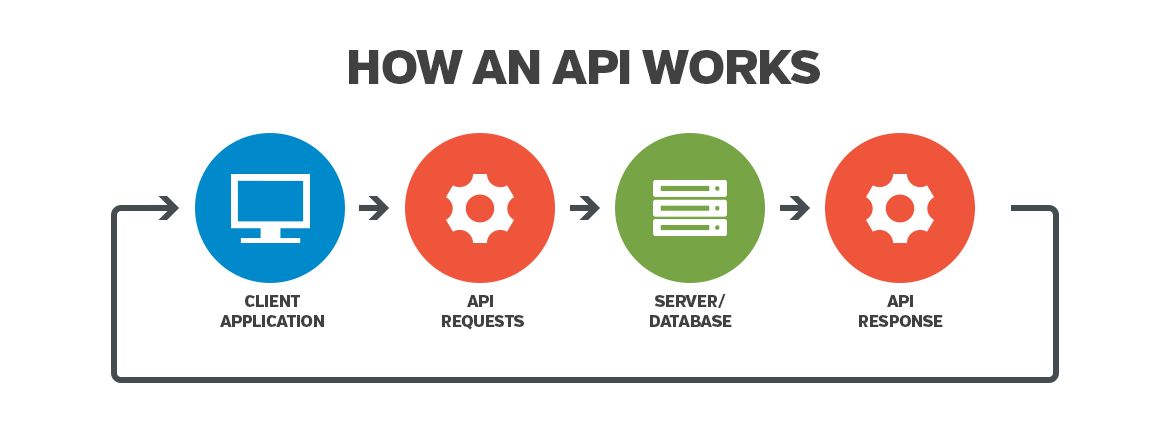
\includegraphics[width=5in]{latex/figures/API.png}
            \captionsource{การทํางานของ API}{\url{https://blog.calameo.com/2744/api-quick-guide/}}
        \end{figure}



\subsection{ความสําคัญของ API}
    ในยุคก่อนที่จะมี API หากผู้ใช้อินเทอร์เน็ตต้องการที่จะเข้าถึงแอปพลิเคชันหรือ service
ที่แตกต่างกันหลาย ๆ รายการ จําเป็นต้องเชื่อมต่อแยกทีละรายการ แต่ในปัจจุบันนี้ เพียงแค่ใช้\mbox{ซอฟต์แวร์}
ตัวเดียวก็สามารถเชื่อมต่อรายการทั้งหมดได้ในช่วงเวลาเดียวกัน โดยข้อดีของ API สามารถแบ่งได้เป็น
3 ข้อ ดังนี้

     \begin{enumerate}
    \item ใช้ API ลดขั้นตอนในการทํางาน ยกตัวอย่างเช่น ในบางกรณีที่ผู้ใช้ต้องการเช็คข้อมูลข่าวสาร
จากเว็บไซต์ หรือแอปพลิเคชัน Facebook และ Twitter หากไม่ใช้ API ผู้ใช้จําเป็นต้องทําการ
เข้าเว็บไซต์ทั้งสองเว็บไซต์ และตรวจสอบข้อมูลแยกกัน แต่หากใช้แอปพลิเคชันที่มี API เช่น The Sprout Social ที่จะรวมหน้ากระดานข่าว (feed) ของทั้ง Facebook และ Twitter อยู่ในที่ ๆ เดียวกัน ทําให้ประหยัดเวลาในการค้นหาข่าวสารหรือการแจ้งเตือนของแต่ละ\mbox{แอปพลิเคชัน}
    \item ใช้ API เพื่ออํานวยความสะดวกในชีวิตประจําวัน เช่น กรณีของสถานีรถไฟฟ้าที่จะมีป้ายบอก
กําหนดเวลาที่รถไฟฟ้าขบวนต่อไปจะมาถึง ในกระบวนการดังกล่าวมีการใช้ API เพื่อให้ผู้โดย สารสามารถคาดการณ์เวลาที่จะขึ้นรถไฟฟ้าได้
    \item ใช้ API เพื่อขยายฐานทางธุรกิจ หรือการที่ผู้พัฒนาต้องการขยายผลประกอบการหรือชิ้นงาน
ซอฟต์แวร์ต่าง ๆ ให้ผู้พัฒนาในธุรกิจเดียวกัน สามารถทําได้เพื่อย่นระยะเวลาในการทํางาน
\end{enumerate}


\section{REST API}
    REST API หรือ Representational State Transfer API \cite{Rest} เปรียบเสมือนเส้นทางที่ระบบ
คอมพิวเตอร์สองฝั่ง คือฝั่งผู้ส่งและฝั่งผู้รับ จะทําการติดต่อสื่อสารกันผ่าน HTTP protocol ใน
ลักษณะเดียวกันกับการติดต่อสื่อสารระหว่าง web browser และ server โดยการติดต่อรับส่งข้อมูลระหว่างระบบนับเป็นพื้นฐานของการพัฒนาซอฟต์แวร์เช่นกัน
\subsection{ข้อจํากัดและส่วนประกอบของ REST และ REST API}
    REST ถูกกําหนดขึ้นในปี 2000 โดย Roy Fielding เพื่อให้เป็นมาตรฐานและใช้งานได้ง่าย แต่ในขณะเดียวกันก็นับเป็นข้อจํากัดที่จําเป็นในการทําRESTful web services โดย REST API มีคุณลักษณะดังนี้

\begin{enumerate}
    \item Client-Server คือ การที่ระบบหนึ่งส่งข้อมูลหรือ request ผ่าน HTTP ไปบน URL ที่อีกระบบหนึ่งเป็นเจ้าของ โดยระบบที่เป็นเจ้าของ URL นั้นจะทําการส่งข้อมูลกลับมา เรียกว่า response ซึ่งการทํางานในลักษณะนี้ถูกใช้ในชีวิตประจําวันในรูปแบบของ web browser คือแอปพลิเคชันส่ง request ไปที่ URL หนึ่ง ๆ ซึ่งเป็นเส้นทางสู่ web server ที่จะส่งข้อมูลกลับมาเป็นหน้า HTML page ซึ่งในหน้า page นั้นอาจมี references ต่างๆเชื่อมอยู่มากมาย เช่น รูปภาพ, style sheet หรือรูปแบบของ JavaScript ที่เป็นผลกระทบเกิดขึ้นจาก request และ response

    \item Stateless คือ ไม่มีการจดจําสถานะ โดย request ของผู้ใช้ (client) สมควรที่จะมีข้อมูลเพียงพอที่จะสามารถ respond ได้ กล่าวคือ เป็นไปได้ที่จะมี HTTP request ในจํานวนที่มากกว่า 1 request ที่สามารถได้รับ respond รูปแบบเดียวกันได้
    \item Cacheable คือ ค่า response ควรที่จะเก็บเป็น Cache ได้ กล่าวคือ สามารถเก็บค่า response ไว้เป็นข้อมูลชั่วคราวในที่เก็บข้อมูลชั่วคราวเพื่อเรียกใช้ในภายหลังได้
    \item Layered คือ ผู้ใช้ที่ทําการส่ง request ไม่จําเป็นต้องรู้ถึงเบื้องลึกของการสื่อสารกับ server เช่น proxy หรือตัวกลางอื่น ๆ

\end{enumerate}

\subsection{Golang Framework}
    จากการศึกษางานที่เกี่ยวของเกี่ยวกับการพัฒนา REST API ผู้จัดทำได้คัดเลือก 
framework ที่จะนำมาพัฒนา API ในโครงงานนี้โดยคัดเลือกมาทั้งหมด 3 อันได้แก่
\begin{enumerate}
    \item Gin พัฒนามาจาก Martini ใช้ customized version ของ HTTP router package 
เพื่อความ เร็วของ Web Application
        \begin{enumerate}[\theenumi.\arabic*]
            \item ข้อดี – มี feature หรือ libraries ที่สำคัญเหมาะกับ service ที่มีขนาดเล็กไม่มีความ
ซับซ้อนมาก มีการแบ่งกลุ่ม API เพื่อความสะดวกในการใช้งาน
            \item ข้อเสีย – ไม่เหมาะกับโปรเจคที่มีขนาดใหญ่และความซับซ้อนสูง
        \end{enumerate}
        
    \item Beego มี Feature ต่าง ๆ ที่มักใช้งานในเว็บแอปพลิเคชันโดยถูกจัดออกเป็น 
Module \mbox{ต่าง ๆ} \mbox{8 Modules} ที่เราสามารถเปิดใช้หรือปิดมันได้ตามต้องการ และยังมี object relationship map (ORM) สำหรับการเข้าถึงข้อมูล, built-in cache handler, session handling tools, logging mechanisms และ libraries สำหรับ operations ทั่วไปกับ HTTP 
objects นอกจากนี้ยังมี command-line tools อีกด้วย
        \begin{enumerate}[\theenumi.\arabic*]
            \item ข้อดี – ไม่จำเป็นต้องหา libraries จากภายนอก และเป็นมิตรต่อผู้ใช้งาน
            \item ข้อเสีย – เก็บ caches ไว้ทำให้ตอนเกิด error จึงดูไม่ออก
        \end{enumerate}

    \item Revel เป็น framework ที่มีพื้นฐาน MVC และยังสามารถเพิ่ม components อื่น ๆ 
ได้อย่างอิสระเพื่อตอบสนองความต้องการของผู้ใช้
        \begin{enumerate}[\theenumi.\arabic*]
            \item ข้อดี – มีความยืดหยุ่นในการใช้งาน การจัดการ database ก็สามารถใช้ข้างนอกได้
            \item ข้อเสีย – ไม่มีตัวจัดการ database เอง
        \end{enumerate}
\end{enumerate}
จากที่ได้ข้อมูลผู้จัดทำพิจารณา ข้อมูลของ framework , ข้อดีและข้อเสียของแต่ละ framework แล้ว จึงเลือกใช้เป็น Gin framework เพราะมีประสิทธิภาพการใช้งานที่สูง และโครงงานที่เราจัดทำเป็น microservice ซึ่งเป็นจุดเด่นของ Gin framework และด้วยความที่มีการใช้งานอย่างแพร่หลายมีข้อมูลให้ศึกษามาก จึงสะดวกในการศึกษาพัฒนาให้เกิดประโยชน์ของเว็บแอปพลิเคชันสูงสุด
\section{Open API}
    OpenAPI หรือ OpenAPI specification เป็นตัวที่จะช่วยให้การพัฒนาแอพพลิเคชันที่มี 
protocol หลายตัว, interface จํานวนมาก รวมถึง environment ต่าง ๆ สามารถพัฒนาได้ง่ายมากยิ่งขึ้น โดยรวมเป็น interface เพียง interface เดียวที่สามารถเข้าถึงข้อมูลภายในได้

\subsection{ความหมายของ OpenAPI Specification}
    OpenAPI Specification หรือที่ในอดีตคือ Swagger Specification เป็น open-sorce
format และถูกสร้างขึ้นเพื่อการออกแบบไฟล์ interface สําหรับให้คอมพิวเตอร์อ่าน (machine-readable)
ที่ถูกใช้ในการผลิต, กําหนด, สํารวจและใช้งาน RESTful API และ web service ต่าง ๆ โดยไฟล์
OpenAPI จะอนุญาติให้นักพัฒนาสามารถระบุสิ่งจําเป็นสําหรับ API นั้น ๆ ได้ คือ
\begin{itemize}[\textbullet]
    \item กําหนด endpoint และ คําสั่งของแต่ละ endpoint
    \item ตัวแปร parameters ของคําสั่ง input และ output
    \item รูปแบบการยืนยันตัวตน
    \item ข้อมูลอื่น ๆ เช่น การติดต่อ, terms of use และ license
\end{itemize}
\subsection{การทํางานของ OpenAPI}
    นอกจากช่วยเหลือผู้ใช้ให้สามารถการเชื่อมต่อกับ remote service ต่าง ๆ โดยง่ายแล้ว
ยังสามารถใช้ OpenAPI ในการทํางานส่วนอื่น ๆ ได้ ดังนี้
        \begin{enumerate}
            \item Generate server สําหรับ API
            \item Generate library ของผู้ใช้งานสําหรับ API โดยใน library มีมากกว่า 40 ภาษา
            \item ใช้งาน specification เพื่อเข้าถึงเครื่องมือต่างๆของ API
            \item สร้าง interactive API documentation ที่ทําให้ user สามารถทดลองเรียก API ได้ผ่านทางเบราว์เซอร์ โดยตรง
            \item สามารถถูกเรียกใช้โดยเครื่องมือ generate code เพื่อ generate server SDK และ CDKs ของผู้ใช้ได้ในหลาย ๆ ภาษา รวมไปถึงเครื่องมือที่ใช้ test อื่น ๆ
        \end{enumerate}

        \begin{figure}[H]
            \centering
                \centering
                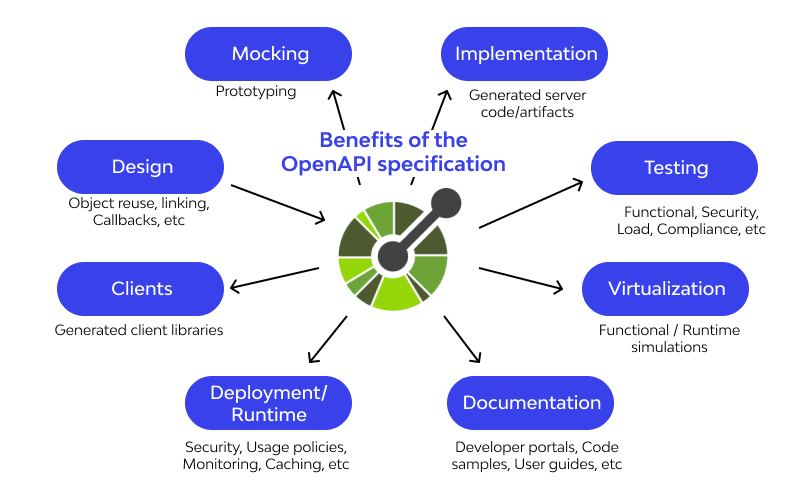
\includegraphics[width=5in]{latex/figures/openapi.png}
            \captionsource{การทํางานของ OpenAPI}{\url{https://www.wallarm.com/what/what-is-openapi}}
        \end{figure}

      

